\paragraph{}
La planificación realizada para el desarrollo del proyecto, está dividida en varias partes:

%\begin{itemize}
%    \item \textbf{Fase inicial}: la primera fase consistió en plantear la idea del proyecto, con la ayuda del tutor. Tras varias
%    propuestas realizadas y la deliveración sobre las mismas, se decidió realizar este proyecto.
%    
%    \item \textbf{Fase de análisis}: durante esta etapa se realizó la especificación de los requisitos
%    \item \textbf{}:
%    \item \textbf{}:
%    \item \textbf{}:
%    \item \textbf{}:
%\end{itemize}

\section{Fase inicial}

\paragraph{}
La primera fase consistió en plantear la idea del proyecto, con la ayuda del tutor. Tras varias
propuestas y la deliberación sobre las mismas, se decidió realizar este proyecto.

\paragraph{}
También se pensó en que lenguaje se desarrollaría el proyecto, así como las principales bibliotecas
que se usarían durante la realización del mismo.

\section{Fase de análisis}

\paragraph{}
Esta etapa está dividida principalmente en las dos partes siguiente:

\begin{itemize}
    \item \textbf{Especificación de los requisitos}: estudio de los requisitos que deberá cumplir el juego.
    
    \item \textbf{Recurso necesarios}: recursos necesarios que deberemos usar durante el desarrollo del proyecto.
\end{itemize}

\section{Fase Aprendizaje}

\paragraph{}
Dado que el proyecto se realizaría con un lenguaje de programación del que no se tenían conocimientos, en este caso \emph{Python}, 
así como de la biblioteca que usaríamos en el desarrollo, como es \emph{Pygame}, esta fase se dividió en dos partes:

\begin{itemize}
    \item \textbf{Aprendizaje de \emph{Python}}: periodo empleado para el aprendizaje del lenguaje de programación \emph{Python},
    durante esta etapa se consultó varios libros sobre lenguaje, así como foros de internet y páginas web. Para un aprendizaje más
    ameno y llevadero, se realizaron problemas ya resuelto en otros lenguajes.
    
    \item \textbf{Familiarización con la biblioteca \emph{Pygame}}: tras el periodo de aprendizaje del lenguaje, debía familiarizarme
    con la biblioteca principal que se usaría en el desarrollo del proyecto, como es \emph{Pygame}. Durante su
    aprendizaje se realizaron pequeñas aplicaciones sencillas, para asentar
    bien los conocimientos.
\end{itemize}

\section{Fase de desarrollo}

\paragraph{}
Tras la consecución de las etapas anteriores, se comenzó el desarrollo del proyecto. Esta etapa del desarrollo es la más extensa de 
todas, como es comprensible. Y también la etapa que más subetapas contiene, las principales son la siguientes:

\begin{itemize}
    \item \textbf{Motor básico}: implementación de las necesidades básicas del proyecto, como control del teclado, carga de recursos, movimiento
    de los vehículos.
    
    %\item \textbf{Movimiento de vehículos}: relización del movimiento y comportamiento que deberían tener los vehículos: giro, 
    %aceleración, frenada.
    
    \item \textbf{Carga de escenario}: carga de los circuitos que compondrán el juego de forma que no fuera necesario tocar código
    para la ampliación del juego.
    
    \item \textbf{Creación de menús}: implementación de toda la interfaz de menús de la que estaría compuesto el juego, menú de 
    opciones, selección de personaje, selección de circuito, etc.
    
    \item \textbf{Colisiones}: unos de los aspectos más básico y esenciales de cualquier juego, se debía implementar las colisiones con el
    escenario, así como con otros elementos del juego como pueden ser ítems u otros vehículos.
    
    \item \textbf{Ítems}: implementación del comportamiento y efecto que
    producirían cada uno de los ítems que están disponibles en el juego.
    
    \item \textbf{Inteligencia artificial}: planteamiento y desarrollo de los vehículos que serían manejados por la inteligencia 
    artificial, estos deberían de se capaces de evitar obstáculos, realizar
    recorridos y lanzar ítems.
    
    \item \textbf{Modos de juego}: realización de los modos de juego que componen el proyecto, como serían carrera rápida, contrarreloj
    y campeonato,
\end{itemize}

\section{Pruebas y correcciones}

\paragraph{}
Una de las etapas más importantes, si no es la que más, del desarrollo de cualquier proyecto. Esta etapa se realizaría en paralelo
a la de desarrollo, ya que conforme se implementan nuevas funcionalidades, cada
un debía ser probada exhaustivamente en cualquiera
de las posibles situaciones que pudiera suceder.

\section{Diagrama de Gantt}

\paragraph{}
A continuación se muestra la planificación anteriormente comentada, en su correspondiente diagrama de Gantt:

\begin{figure}[H]
  \label{gant1}
  \begin{center}
    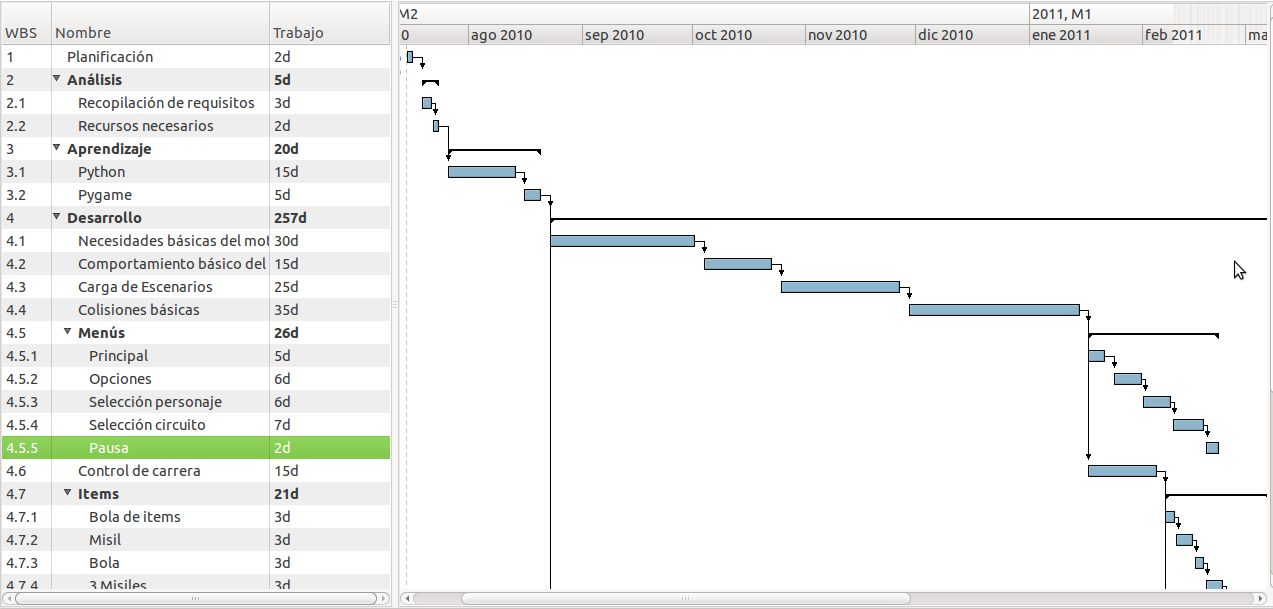
\includegraphics[scale=0.51, angle=90]{imagenes/planificacion/gant1.png}
  \end{center}
  \caption{Planificación: Diagrama de Gantt 1/2.}
\end{figure}

\begin{figure}[H]
  \label{gant2}
  \begin{center}
    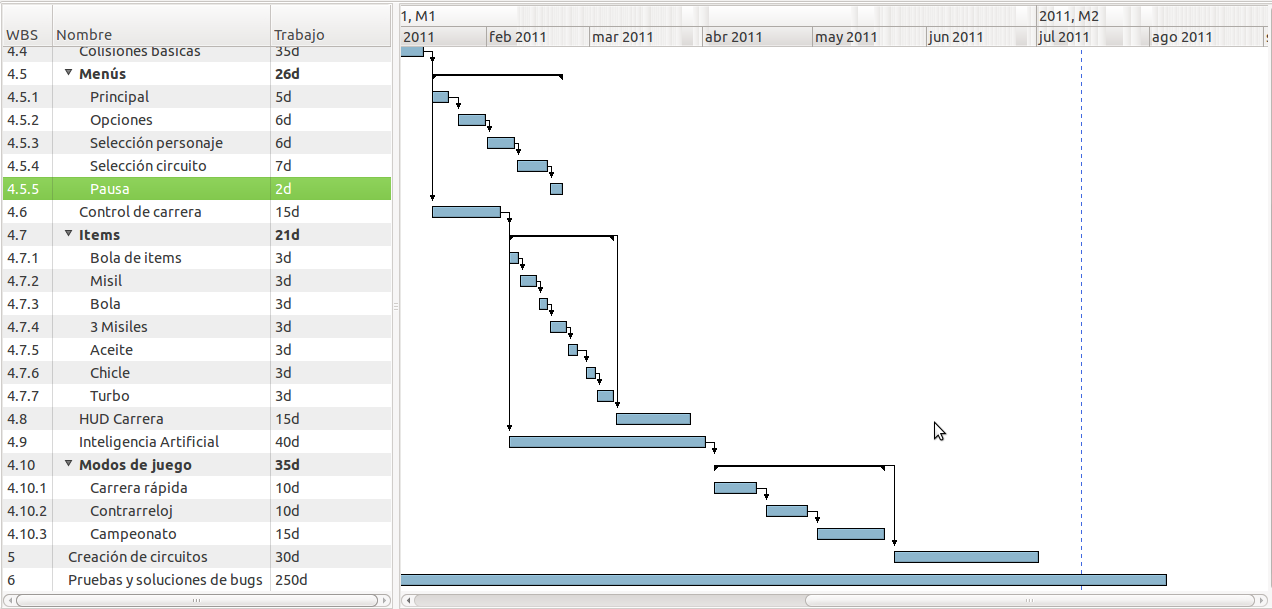
\includegraphics[scale=0.51, angle=90]{imagenes/planificacion/gant2.png}
  \end{center}
  \caption{Planificación: Diagrama de Gantt 2/2.}
\end{figure}
